\documentclass{ximera}
%% You can put user macros here
%% However, you cannot make new environments

\listfiles

\graphicspath{{./}{firstExample/}{secondExample/}}

\usepackage{tikz}
\usepackage{tkz-euclide}
\usepackage{tikz-3dplot}
\usepackage{tikz-cd}
\usetikzlibrary{shapes.geometric}
\usetikzlibrary{arrows}
\usetkzobj{all}
\pgfplotsset{compat=1.13} % prevents compile error.

%\renewcommand{\vec}[1]{\mathbf{#1}}
\renewcommand{\vec}{\mathbf}
\newcommand{\RR}{\mathbb{R}}
\newcommand{\dfn}{\textit}
\newcommand{\dotp}{\cdot}
\newcommand{\id}{\text{id}}
\newcommand\norm[1]{\left\lVert#1\right\rVert}
 
\newtheorem{general}{Generalization}
\newtheorem{initprob}{Exploration Problem}

\tikzstyle geometryDiagrams=[ultra thick,color=blue!50!black]

%\DefineVerbatimEnvironment{octave}{Verbatim}{numbers=left,frame=lines,label=Octave,labelposition=topline}



\usepackage{mathtools}


\author{}
\title{Picture Perfect} \license{CC BY-NC-SA 4.0}
\begin{document}

\begin{abstract}
Students simulate a manufacturing process by tearing paper into rectangles, performing measurements, recording, and analyzing their data.
\end{abstract}
\maketitle

\begin{onlineOnly}
\section*{Picture Perfect: A Data Collection Activity}
\end{onlineOnly}

\subsection*{Evaluating an Existing Process}

Suppose you have been called in to evaluate the process of manufacturing small picture frames.  A picture frame typically consists of the frame, a piece of glass, and a fiberboard back that holds the picture in place. The photo below shows the kind of picture frame the shop manufactures. Note that the fiberboard back is held in place by metal tabs.  

\begin{center}
         \begin{tikzpicture}
 \node[inner sep=0pt, anchor=base] (p1) at (0,0)
   {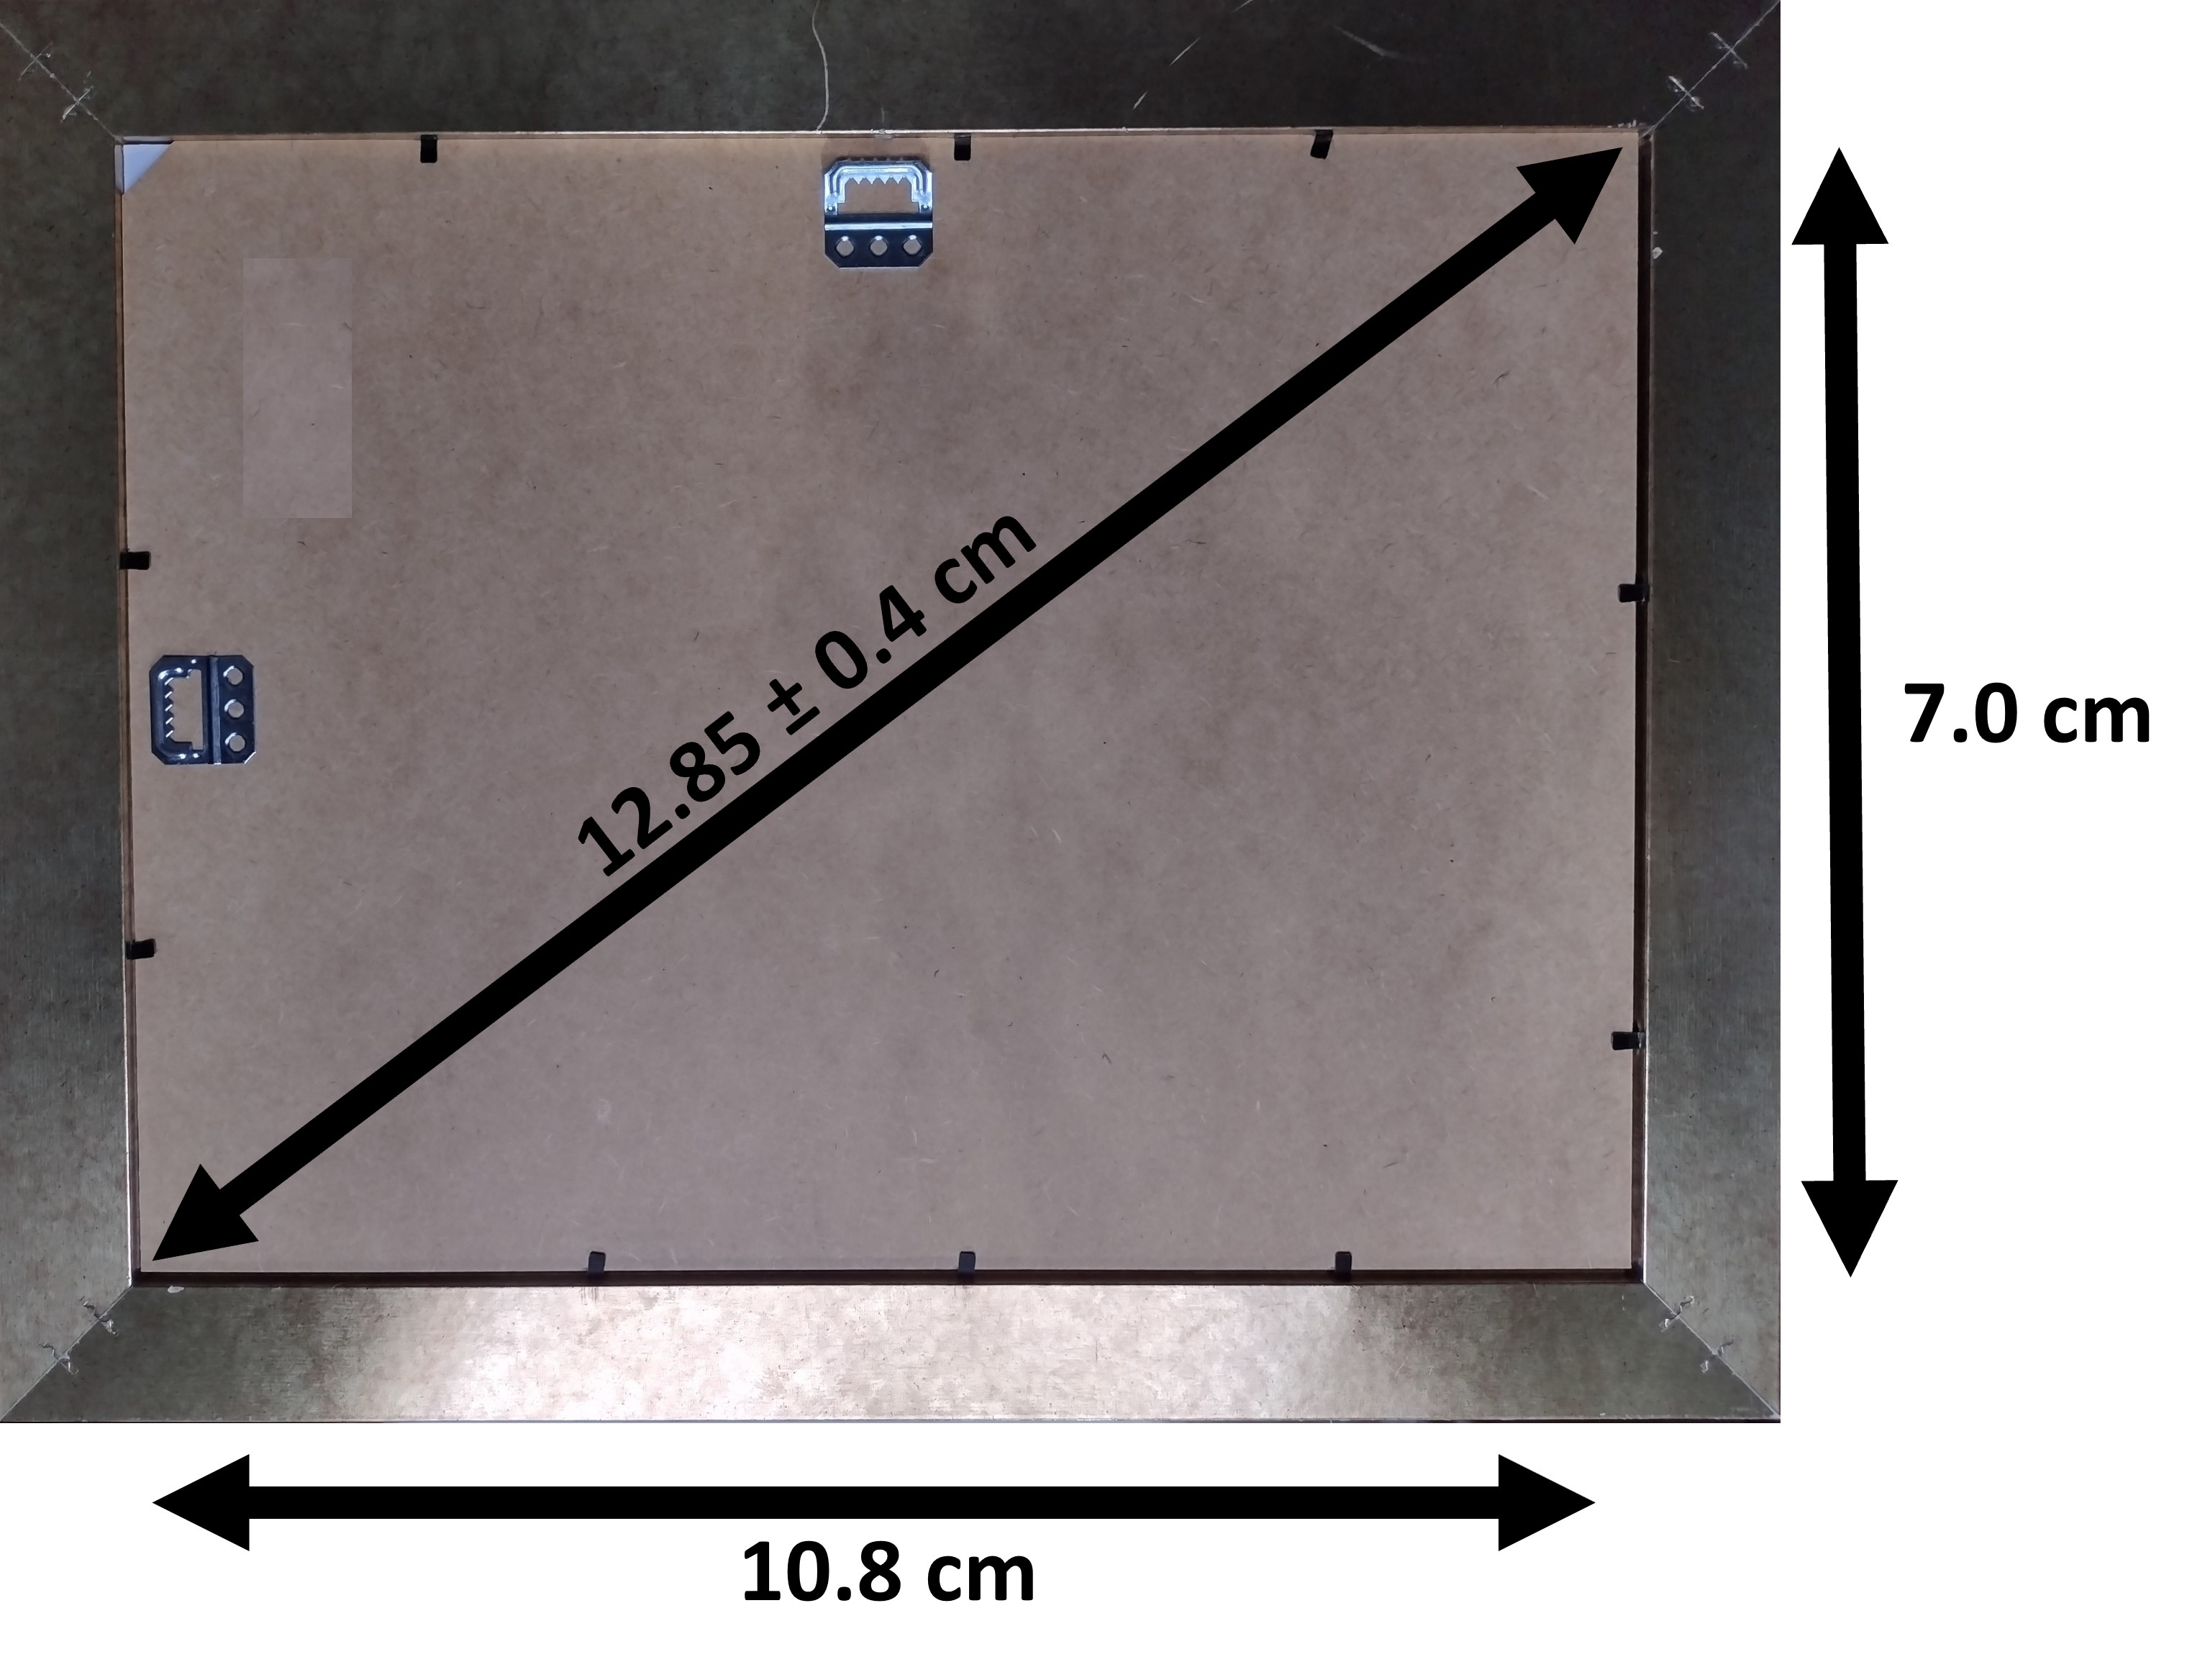
\includegraphics[height=80mm]{frame.jpg}};
               \end{tikzpicture}
       \end{center}

The shop owner is concerned about the quality of the fiberboard backs.  The target size for the back is $7$cm $\times$ $10.8$cm, with a $12.85$cm diagonal (diagonal length has been rounded to the nearest half a millimeter).  The fiberboard has to be small enough to fit into the frame, but big enough to not to slip out of the tabs.  This dictates the specification limits.  Suppose the specs for the diagonal are set to be $12.85\pm 0.4$cm.

\begin{question}\label{quest:qc150_1}
What are the lower and upper specification limits in cm for the diagonal dimension?

Lower Specification Limit (LSL) $=\answer{12.45}\text{cm}$

Upper Specification Limit (USL) $=\answer{13.25}\text{cm}$

\end{question}

\begin{question}\label{quest:qc150_2}
    Consider the population of fiberboard backs.  The manufacturing process will naturally result in some variability in the length of the diagonal.  If everything is under control, the diagonal measurements will be approximately normally distributed.  Use LSL and USL values from the previous problem to select the most appropriate target mean and standard deviation for the distribution of the diagonal lengths, if we want to have $Cp=Cpk=1.33$.

    \begin{multipleChoice}
        \choice[correct]{$\mu=12.85$, $\sigma= 0.1$}
        \choice{$\mu=12.85$, $\sigma= 0.15$}
        \choice{$\mu=12.85$, $\sigma= 0.4$}
        \choice{$\mu=12.85$, $\sigma= \pm 0.4$}
    \end{multipleChoice}
\end{question}

Currently, the fiberboard backs are being cut by two different machines.  We will call them Machine 1 and Machine 2.
Enter the lower and upper spec limits for the diagonal measurements into the GeoGebra interactive below.  Use the check boxes to display the histograms for the diagonal length measurements for large batches of output produced by Machine 1 and Machine 2. 

\begin{onlineOnly}
\begin{center} 
\geogebra{ajtk6jux}{950}{600} 
\end{center}
\end{onlineOnly}

\begin{question}\label{quest:Mach1Mach2}
\begin{hint}
    $Cp=\frac{\text{Spec Width}}{\text{Process Width}}=\frac{\text{Upper Spec Limit}-\text{Lower Spec Limit}}{6\sigma}$, and $Cpk=\frac{\text{Distance from Mean to the nearest Spec Limit}}{3\sigma}$
\end{hint}
How would you characterize the output from Machine 1? Check ALL that apply.

\begin{selectAll}
\choice{The process is accurate}
\choice{The process is precise}
\choice[correct]{There is a lot of scrap}
\end{selectAll}

What can you say about $Cp$ for Machine 1?

\begin{selectAll}
\choice{$Cp>1$}
\choice[correct]{$Cp<1$}
\choice{$Cp=1$}
\end{selectAll}

How would you characterize the output from Machine 2? Check ALL that apply.

\begin{selectAll}
\choice{The process is accurate}
\choice[correct]{The process is precise}
\choice{There is a lot of scrap}
\end{selectAll}

What can you say about $Cp$ and $Cpk$ for Machine 2?  Check ALL that apply.

\begin{selectAll}
\choice[correct]{$Cp>1$}
\choice{$Cp<1$}
\choice{$Cp=1$}
\choice{$Cp=Cpk$}
\choice[correct]{$Cp>Cpk$}
\choice{$Cp<Cpk$}
\end{selectAll}
\end{question}

\subsection*{Changing Fiberboard Suppliers}

The dimensions of the frame are given in centimeters, per customer request. Suppose your shop gets a new fiberboard supplier who offers 8.5in $\times$ 11in pieces of fiberboard.  The shop manager suggests that if you cut each piece of fiberboard into eight equal rectangles, as shown below, the result will be ``close enough".

\begin{center}
\begin{tikzpicture}[scale=0.5]
\draw[black, thick, fill=yellow,opacity=0.25] (-1,-1) rectangle (23, 9.5);
 \draw[black, thick, fill=white] (0,0) rectangle (11,8.5);
 \draw[line width=0.5pt, dashed, gray](5.5,0)--(5.5,8.5);
  \draw[line width=0.5pt, dashed, gray](2.75,0)--(2.75,8.5);
   \draw[line width=0.5pt, dashed, gray](8.25,0)--(8.25,8.5);
    \draw[line width=0.5pt, dashed, gray](0,4.25)--(11,4.25);
%\node[rotate=90] at (5,4.5)   {fold and tear line};
\draw[line width=1pt,gray, stealth-](0,-0.5)--(4,-0.5);
\draw[line width=1pt,gray, -stealth](7,-0.5)--(11,-0.5);
\node[gray] at (5.5,-0.5)   {11 in};
\draw[line width=1pt,gray, -stealth](-0.5,2.75)--(-0.5,0);
\draw[line width=1pt,gray, -stealth](-0.5, 5.75)--(-0.5, 8.5);
\node[rotate=90, gray] at (-0.5,4.25)   {8.5 in};

\draw[black, thick, fill=white] (17.75,2.75) rectangle (20.5, 7);
\draw[black, thick, fill=white] (17.5,2.5) rectangle (20.25, 6.75);
\draw[black, thick, fill=white] (17.25,2.25) rectangle (20, 6.5);
\draw[black, thick, fill=white] (17,2) rectangle (19.75, 6.25);
\draw[black, thick, fill=white] (16.75,1.75) rectangle (19.5, 6);
\draw[black, thick, fill=white] (16.5,1.5) rectangle (19.25, 5.75);
\draw[black, thick, fill=white] (16.25,1.25) rectangle (19, 5.5);
 \draw[black, thick, fill=white] (16,1) rectangle (18.75, 5.25);

 \draw[line width=1pt,gray, stealth-](17.75,7.5)--(19,7.5);
\draw[line width=1pt,gray, -stealth](19,7.5)--(20.5,7.5);
\node[gray] at (19.25,8)   {2.75 in};
\draw[line width=1pt,gray, stealth-](21,2.75)--(21,6);
\draw[line width=1pt,gray, -stealth](21, 6)--(21, 7);
\node[rotate=90, gray] at (21.5,4.9)   {4.25 in};

\end{tikzpicture}

\end{center}

% Our best customer placed an order for 100 units of product.  The product is rectangular sheets of silicon that will be sent through a stamping operation to create round wafers. These silicon wafers will be used to manufacture integrated circuit chips. The silicon sheets will be $6.98$cm by $10.79$cm ($2.75$in $\times$ $4.25$in) with a nominal diagonal dimension of $12.85$cm ($5.06$in).  To properly align in the stamping machine, the diagonal specifications must be $12.85$cm $\pm$ $0.15$cm  ($5.06$in $\pm$ $0.06$in).



\begin{question}\label{quest:qc150_3}
    Is the shop manager being reasonable?  Convert the  dimensions of fiberboard backs to centimeters to find out.  Enter your answers to three decimal places.

    $$2.75\text{in}=2.75\text{in}\times \frac{2.54\text{cm}}{\text{in}}=\answer{6.985}\text{cm}$$
    $$4.25\text{in}=4.25\text{in}\times \frac{2.54\text{cm}}{\text{in}}=\answer{10.795}\text{cm}$$
\end{question}

\subsection*{Data Collection Activity}
You will simulate this manufacturing process using $8.5$in $\times$ $11$in sheets of paper.

\textbf{Supplies needed:}
\begin{itemize}
\item A total of 16 or more sheets of standard copier paper 21.59cm $\times$ 27.94cm (8.5in $\times$ 11in) to be evenly distributed among groups of 2 - 4 students. The paper will be used in place of fiberboard.  
\item Each group will need a 30.48cm (12-inch) ruler. Note that measurements will be recorded in cm.  \href{http://www.vendian.org/mncharity/dir3/paper_rulers/}{Here is a printable ruler.}  Select the first ruler in the list.
\item Google Sheets spreadsheet that every group can access to enter data.  (Instructor needs to create and share an editable link with the class.)
\end{itemize}

\textbf{Procedure:}
\begin{enumerate}
\item	Break up into small groups (2 - 4 students per group).    Group members will take on the following roles:
    \begin{itemize}
\item A paper-folder
\item A paper-tearer
\item A measurer
\item A data recorder 
\item All students will serve as statistical analysts.
    \end{itemize}
    
\item Carefully fold and tear each sheet of paper as indicated by the dashed lines in the diagram below.

\begin{center}
\begin{tikzpicture}[scale=0.5]
\draw[black, thick, fill=yellow,opacity=0.25] (-1,-1) rectangle (26, 10.5);
 \draw[black, thick, fill=white] (0,0) rectangle (11,8.5);
 \draw[line width=0.5pt, dashed, gray](5.5,0)--(5.5,8.5);
\node[rotate=90] at (5,4.5)   {fold and tear line};
\draw[line width=1pt,gray, stealth-](0,-0.5)--(4,-0.5);
\draw[line width=1pt,gray, -stealth](7,-0.5)--(11,-0.5);
\node[gray] at (5.5,-0.5)   {11 in};
\draw[line width=1pt,gray, -stealth](-0.5,2.75)--(-0.5,0);
\draw[line width=1pt,gray, -stealth](-0.5, 5.75)--(-0.5, 8.5);
\node[rotate=90, gray] at (-0.5,4.25)   {8.5 in};

\draw[black, thick, fill=white] (13,0) rectangle (18.5,8.5);
\draw[black, thick, fill=white] (19.5,0) rectangle (25,8.5);
 \draw[line width=0.5pt, dashed, gray](13,4.25)--(18.5,4.25);
  \draw[line width=0.5pt, dashed, gray](19.5,4.25)--(25,4.25);
 \node[] at (15.75,4.75)   {tear line};
  \node[] at (22.25,4.75)   {tear line};
%  \draw[line width=1pt,gray, stealth-](19.5,-0.5)--(21,-0.5);
% \draw[line width=1pt,gray, -stealth](23.75,-0.5)--(25,-0.5);

\node[] at (5.5,9.5)   {\Large{Step 1}};
\node[] at (19,9.5)   {\Large{Step 2}};
\end{tikzpicture}

\begin{tikzpicture}[scale=0.5]
 \draw[black, thick, fill=yellow,opacity=0.25] (-1,-1) rectangle (26, 11.5);
 \draw[black, thick, fill=white] (0,0) rectangle (5.5, 4.25);
 \draw[black, thick, fill=white] (6.5,0) rectangle (12,4.25 );
  \draw[black, thick, fill=white] (0,5.25) rectangle (5.5, 9.5);
   \draw[black, thick, fill=white] (6.5,5.25) rectangle (12, 9.5);

  \draw[line width=0.5pt, dashed, gray](2.75,5.25)--(2.75,9.5);
\draw[line width=0.5pt, dashed, gray](2.75,0)--(2.75,4.25);
\draw[line width=0.5pt, dashed, gray](9.25,0)--(9.25,4.25);
\draw[line width=0.5pt, dashed, gray](9.25,5.25)--(9.25,9.5);
  
\node[rotate=90] at (2.25,2.13)   {tear line};
\node[rotate=90] at (2.25,7.38)   {tear line};
\node[rotate=90] at (8.75,2.13)   {tear line};
\node[rotate=90] at (8.75,7.38)   {tear line};

\draw[black, thick, fill=white] (17.75,2.75) rectangle (20.5, 7);
\draw[black, thick, fill=white] (17.5,2.5) rectangle (20.25, 6.75);
\draw[black, thick, fill=white] (17.25,2.25) rectangle (20, 6.5);
\draw[black, thick, fill=white] (17,2) rectangle (19.75, 6.25);
\draw[black, thick, fill=white] (16.75,1.75) rectangle (19.5, 6);
\draw[black, thick, fill=white] (16.5,1.5) rectangle (19.25, 5.75);
\draw[black, thick, fill=white] (16.25,1.25) rectangle (19, 5.5);
 \draw[black, thick, fill=white] (16,1) rectangle (18.75, 5.25);

 \draw[line width=1pt,gray, stealth-](17.75,7.5)--(19,7.5);
\draw[line width=1pt,gray, -stealth](19,7.5)--(20.5,7.5);
\node[gray] at (19.25,8)   {2.75 in};
\draw[line width=1pt,gray, stealth-](21,2.75)--(21,6);
\draw[line width=1pt,gray, -stealth](21, 6)--(21, 7);
\node[rotate=90, gray] at (21.5,4.9)   {4.25 in};

\node[] at (5.75,10.5)   {\Large{Step 3}};
\node[] at (19,10.5)   {\Large{Step 4}};
\end{tikzpicture}
\end{center}

At the end of the process you will have eight small rectangles for every sheet of paper, as shown in Step 4.  (If your class used a total of 16 pages, then a total of 104 rectangles should have been produced.  Larger classes may use more paper and produce more rectangles.)

\item Carefully measure the diagonal of each rectangle in centimeters and record your measurement to the nearest half a millimeter.  (This means that a measurement that falls between 12.7 and 12.8 cm will get recorded as 12.75 cm.)
\item Access a Google Sheets document through the link shared by your instructor and record your diagonal measurements.  The screenshot below shows what the Google Sheets set-up might look like.

\begin{center}
         \begin{tikzpicture}
 \node[inner sep=0pt, anchor=base] (p1) at (0,0)
   {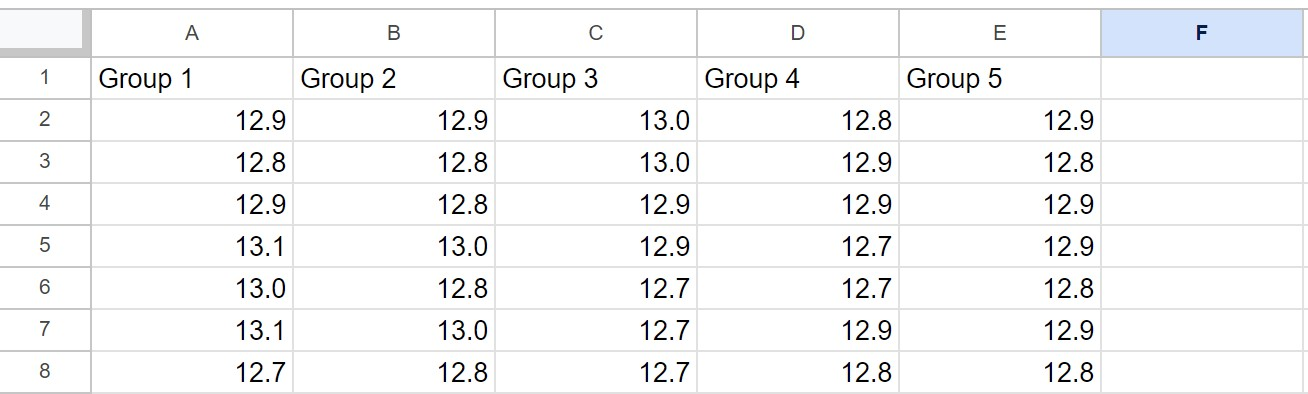
\includegraphics[height=40mm]{classData1.jpg}};
               \end{tikzpicture}
       \end{center}

\item The instructor should combine the data for the entire class by copying and pasting the data from every group into a single column.
\item Students should copy and paste the column of class data from the previous step into column A of the GeoGebra interactive below. (Column A currently contains sample data that needs to be deleted.)  
\end{enumerate}

\begin{onlineOnly}
\begin{center} 
\geogebra{vrdgwu5p}{950}{600} 
\end{center}
\end{onlineOnly}

% \begin{question}
%     Use the Pythagorean Theorem to complete the following expression for the length of the diagonal of the rectangle.  Then find the length of the diagonal to the nearest tenth of an inch.
%     $$2.75^2+\answer{4.25}^2=d^2$$
%     $$d=\answer{5.1}\,\text{in}$$
% \end{question}

% \begin{question}
%     You will be using centimeter rulers to measure the diagonals of the rectangles.  Let's convert the theoretical length of the diagonal to centimeters.  Use the 
%     \end{question}

\textbf{Analysis/Discussion:}

Use the following questions as discussion prompts.  Your answers will vary, depending on the results of your production process.
\begin{enumerate}
\item What is the advantage of drawing a picture of the data (histogram) compared to looking at a list of numbers?
\item Using the histogram, do you estimate that the mean for your data is above the center line, below the center line or around the center line?  Check the ``Student Data Summary" checkbox to see your data summary.  How does your guess based on the histogram compare to what the numbers tell you? 
\item The histogram provides three pieces of information about the data. Comment on each of these as it relates to your data.
    \begin{itemize}
\item The pattern of the data. This is a crude, subjective assessment of the histogram but can be a useful indicator.  If the histogram is normally distributed, then the process is experiencing only common or natural causes of variation. If the histogram is not normally distributed, then the process is likely experiencing unwanted or assignable causes of variation.    
\item The spread of the data compared to specification limits.  If the spread of the data is as wide (or wider) as the specification limits, then the data is not very precise, and the process is likely to be making scrap. Scrap occurs when a measured value is outside the specification limits.
\item The position of the data compared to specification limits. If the histogram is well-centered within the specification limits, then the process is accurate. That is, the process is making product that is close to the nominal or midpoint of the specification range.
    \end{itemize}
\end{enumerate}

We sometimes need to quantify how far our data are away from the expected value.  To do this we use  the following formula.
\begin{formula}\label{form:percentError}
$$\text{Percent error} = \frac{|\text{Measured Value} – \text{Expected Value}|}{\text{Expected Value}} \times 100\%$$
\end{formula}

In the case of the fiberboard backs, the expected value for the diagonal measurement is 12.85 cm.  What is the percent error of the average of your data compared to the expected value?  






\end{document} 